\subsection{Тестирование}

Тестирование является одним из ключевых этапов разработки, направленным на подтверждение корректности работы программы.

Выделяют три основных вида тестирования \refref{ref:testing}:
\begin{itemize}
    \item модульное тестирование;
    \item интеграционное тестирование;
    \item функциональное тестирование.
\end{itemize}

Модульное тестирование или юнит-тестирование позволяет проверить отдельные изолированные компоненты системы.
Направлено на проверку правильности функционирования каждого блока с помощью входных данных и подтверждения соответствия результата теста ожидаемым результатам.

Интеграционное тестирование направлено на проверку корректности взаимодействия нескольких модулей как единой группы.
Интеграционные тесты позволяют выявить проблемы, связанные с зависимостями и обменом информацией между компонентами системы.

Функциональное тестирование -- тип тестирования, который направлен на проверку соответствия работы программы заданной функциональности.
Основная цель -- убедиться, что разработанное программное обеспечение работает правильно и обеспечивает требуемую функциональность.

Проверка корректности работы лексера, парсера, семантического анализатора и исполнителя выполнена с помощью модульных тестов.
Написаны тесты для большинства основных функций.
Некоторые тест-кейсы приведены в таблицах~\ref{t:testCases_infixIntExpr}-13.

Для реализации и запуска тестов в разработанной программе использовалась встроенная среду выполнения Go утилита <<go test>>.
Эта утилита предоставляет удобный и мощный инструмент для создания и выполнения тестов, включая модульные и функциональные тесты.
<<Go test>> позволяет одной командой запускать все реализованные тест-кейсы в проекте и получать результат их выполнения \refref{ref:go-testing}.

% Фрагменты кода тестирования представлены в приложении Д.

В ходе запуска тестирования все тесты выполнились успешно. Результат тестирования представлен на рисунке~\ref{f:testResult}.

\begin{figure}[ht]
    \centering
    \vspace{\toppaddingoffigure}
    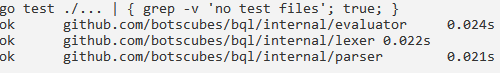
\includegraphics[width=0.9\textwidth]{evaluator/testResult.png}
    \caption{Результаты запуска тестов}
    \label{f:testResult}
\end{figure}

\clearpage

\begin{table}[!ht]
    \Large
    \centering
    \begin{threeparttable}
        \caption{Тест-кейсы исполнения целочисленного выражения}
        \label{t:testCases_infixIntExpr}
        \begin{tabularx}{\textwidth}{|X|c|}
            \hline
            Входные данные                & Ожидаемый результат \\
            \hline
            4                             & 4                   \\
            \hline
            -5                            & -5                  \\
            \hline
            2 + 2                         & 4                   \\
            \hline
            1 + 2 + 3 + 4 + 5 - 1 - 2 - 3 & 9                   \\
            \hline
            2 * 3 * 4 * 5 * 6 * 7 * 8 * 9 & 362880              \\
            \hline
            10 + 10 * 2                   & 30                  \\
            \hline
            (10 + 10) * 2                 & 40                  \\
            \hline
            100 / 2 * 2 + 5               & 105                 \\
            \hline
            100 / (2 * 2) - 200           & -175                \\
            \hline
            5 \% 2                        & 1                   \\
            \hline
            4 \% 2                        & 0                   \\
            \hline
        \end{tabularx}
    \end{threeparttable}
    \vspace{\bottompaddingoftable}
\end{table}

\begin{table}[!ht]
    \Large
    \centering
    \begin{threeparttable}
        \caption{Тест-кейсы исполнения встроенных функций}
        \label{t:testCases_builtins}
        \begin{tabularx}{\textwidth}{|X|c|}
            \hline
            Входные данные            & Ожидаемый результат                        \\
            \hline
            len("abc")                & 3                                          \\
            \hline
            len("abc" + "efg")        & 6                                          \\
            \hline
            len("")                   & 0                                          \\
            \hline
            len(1)                    & type of argument not supported: INTEGER    \\
            \hline
            len("a", "b")             & wrong number of arguments: 2 want: 1       \\
            \hline
            x = "abc"; len(x)         & 3                                          \\
            \hline
            len({[}{]})               & 0                                          \\
            \hline
            x = {[}1, 2, 3{]}; len(x) & 3                                          \\
            \hline
            push({[}{]}, 4)           & {[}4{]}                                    \\
            \hline
            push({[}1, 2, 3{]}, 4)    & {[}1, 2, 3, 4{]}                           \\
            \hline
            push("a", 4)              & first argument must be ARRAY, got: STRING" \\
            \hline
            first({[}{]})             & null                                       \\
            \hline
            first({[}1{]})            & 1                                          \\
            \hline
            first({[}3, 2, 1{]})      & 3                                          \\
            \hline
            first("a")                & argument must be ARRAY, got: STRING        \\
            \hline
            last({[}{]})              & null                                       \\
            \hline
            last({[}1{]})             & 1                                          \\
            \hline
        \end{tabularx}
    \end{threeparttable}
    \vspace{\bottompaddingoftable}
\end{table}

\clearpage

\begin{table}[!ht]
    \Large
    \centering
    \begin{threeparttable}
        \caption{Тест-кейсы семантических ошибок}
        \label{t:testCases_semanticErrors}
        \begin{tabularx}{\textwidth}{|X|c|}
            \hline
            Входные данные                   & Ожидаемый результат                   \\
            \hline
            true + false                     & unknown operator: BOOLEAN + BOOLEAN   \\
            \hline
            1; true - false; 2               & unknown operator: BOOLEAN - BOOLEAN   \\
            \hline
            1; true + false + true + true; 2 & unknown operator: BOOLEAN + BOOLEAN   \\
            \hline
            -true                            & unknown operator: -BOOLEAN            \\
            \hline
            true + 3                         & type mismatch: BOOLEAN + INTEGER      \\
            \hline
            3 * false                        & type mismatch: INTEGER * BOOLEAN      \\
            \hline
            "Hello" * 3                      & type mismatch: STRING * INTEGER       \\
            \hline
            "Hello" * "Earth"                & unknown operator: STRING * STRING     \\
            \hline
            if (3) \{ 1 \}                   & non boolean condition in if statement \\
            \hline
            x = 10; q                        & identifier not found: q               \\
            \hline
            true{[}1{]}                      & index operator not supported: BOOLEAN \\
            \hline
            123{[}123{]}                     & index operator not supported: INTEGER \\
            \hline
        \end{tabularx}
    \end{threeparttable}
    \vspace{\bottompaddingoftable}
\end{table}

\begin{table}[!ht]
    \Large
    \centering
    \begin{threeparttable}
        \caption{Тест-кейсы исполнения вызова функции}
        \label{t:testCases_fnCall}
        \begin{tabularx}{\textwidth}{|X|c|}
            \hline
            Входные данные                                              & Ожидаемый результат \\
            \hline
            x = fn(x)\{ x \}; x(10);                                    & 10                  \\
            \hline
            x = fn(x, y)\{ return x * y \}; x(10, 9);                   & 90                  \\
            \hline
            x = fn(x, y, z)\{ return x * (y - z) \}; x(10,   9, 1);     & 80                  \\
            \hline
            x = fn(x, y)\{ return x + y \}; x(10, x(x(1, 1), x(3, 5))); & 20                  \\
            \hline
            fn(x)\{ x \}(5)                                             & 5                   \\
            \hline
            c = fn(x)\{                                                 & 9                   \\
            fn(y) \{ x + y \}                                           &                     \\
            \}                                                          &                     \\
            a = c(5);                                                   &                     \\
            a(4)                                                        &                     \\
            \hline
        \end{tabularx}
    \end{threeparttable}
    \vspace{\bottompaddingoftable}
\end{table}


\begin{table}[!ht]
    \Large
    \centering
    \begin{threeparttable}
        \caption{Тест-кейсы исполнения массива}
        \label{t:testCases_arrayExprt}
        \begin{tabularx}{\textwidth}{|X|c|}
            \hline
            Входные данные          & Ожидаемый результат \\
            \hline
            {[}1, 2, -33, 5+5, 1 + 2 + 3 + 4 * 5{]}          & {[}1, 2, -33, 10, 26{]}         \\
            \hline
        \end{tabularx}
    \end{threeparttable}
    \vspace{\bottompaddingoftable}
\end{table}

\clearpage

\begin{table}[!ht]
    \Large
    \centering
    \begin{threeparttable}
        \caption{Тест-кейсы исполнения строкового выражения}
        \label{t:testCases_stringExpr}
        \begin{tabularx}{\textwidth}{|X|c|}
            \hline
            Входные данные          & Ожидаемый результат \\
            \hline
            "Hello Earth"           & Hello Earth         \\
            \hline
            "Hello" + " " + "Earth" & Hello Earth         \\
            \hline
        \end{tabularx}
    \end{threeparttable}
    \vspace{\bottompaddingoftable}
\end{table}

\begin{table}[!ht]
    \Large
    \centering
    \begin{threeparttable}
        \caption{Тест-кейсы исполнения булева выражения}
        \label{t:testCases_boolExpr}
        \begin{tabularx}{\textwidth}{|X|c|}
            \hline
            Входные данные              & Ожидаемый результат \\
            \hline
            true                        & true                \\
            \hline
            false                       & false               \\
            \hline
            1 == 1                      & true                \\
            \hline
            1 != 1                      & false               \\
            \hline
            1 \textless 2               & true                \\
            \hline
            1 \textgreater 2            & false               \\
            \hline
            1 \textless{}= 2            & true                \\
            \hline
            1 \textless{}= 1            & true                \\
            \hline
            1 \textgreater{}= 2         & false               \\
            \hline
            1 \textgreater{}= 1         & true                \\
            \hline
            true == true                & true                \\
            \hline
            false == false              & true                \\
            \hline
            true == false               & false               \\
            \hline
            true != false               & true                \\
            \hline
            (true == false) == false    & true                \\
            \hline
            (1 == 1) == true            & true                \\
            \hline
            (1 \textless{}= 1) == false & false               \\
            \hline
            true || false               & true                \\
            \hline
            true \&\& false             & false               \\
            \hline
            true \&\& true              & true                \\
            \hline
            false \&\& false            & false               \\
            \hline
            false || false              & false               \\
            \hline
            !true                       & false               \\
            \hline
            !false                      & true                \\
            \hline
            !!false                     & false               \\
            \hline
        \end{tabularx}
    \end{threeparttable}
    \vspace{\bottompaddingoftable}
\end{table}

\clearpage

\begin{table}[!ht]
    \Large
    \centering
    \begin{threeparttable}
        \caption{Тест-кейсы исполнения условного выражения}
        \label{t:testCases_conditionExpr}
        \begin{tabularx}{\textwidth}{|X|c|}
            \hline
            Входные данные                                 & Ожидаемый результат \\
            \hline
            if (true) \{ 50 \}                             & 50                  \\
            \hline
            if (false) \{ 50 \}                            & null                \\
            \hline
            if (!false) \{ 50 \}                           & 50                  \\
            \hline
            if (1 \textless 2) \{ 50 \} else \{ 100 \}     & 50                  \\
            \hline
            if (1 \textgreater 2) \{ 50 \} else \{ 100 \}  & 100                 \\
            \hline
            if (true || false) \{ 50 \} else \{ 100 \}     & 50                  \\
            \hline
            if (true   \&\& false) \{ 50 \} else \{ 100 \} & 100                 \\
            \hline
        \end{tabularx}
    \end{threeparttable}
    \vspace{\bottompaddingoftable}
\end{table}

\begin{table}[!ht]
    \Large
    \centering
    \begin{threeparttable}
        \caption{Тест-кейсы исполнения индексного выражения для массива}
        \label{t:testCases_arrayIndexExpr}
        \begin{tabularx}{\textwidth}{|X|c|}
            \hline
            Входные данные                                    & Ожидаемый результат \\
            \hline
            {[}1, 2, 5{]}{[}0{]}                              & 1                   \\
            \hline
            {[}1, 2, 5{]}{[}2{]}                              & 5                   \\
            \hline
            {[}1, 2, 5{]}{[}3{]}                              & null                \\
            \hline
            {[}1, 2, 5{]}{[}-1{]}                             & null                \\
            \hline
            {[}1, 2, 5{]}{[}1+1{]}                            & 5                   \\
            \hline
            x = 1; {[}1, 2, 5{]}{[}x{]}                       & 2                   \\
            \hline
            a = {[}1, 2, 5{]}; a{[}0{]} + a{[}1{]} * a{[}2{]} & 11                  \\
            \hline
        \end{tabularx}
    \end{threeparttable}
    \vspace{\bottompaddingoftable}
\end{table}

\begin{table}[!ht]
    \Large
    \centering
    \begin{threeparttable}
        \caption{Тест-кейсы исполнения индексного выражения для хэш-карты}
        \label{t:testCases_HashMapIndexExpr}
        \begin{tabularx}{\textwidth}{|X|c|}
            \hline
            Входные данные                                    & Ожидаемый результат \\
            \hline
            \{"x": 1\}{[}"x"{]}   & 1    \\
            \hline
            \{"x": 1\}{[}"y"{]}   & null \\
            \hline
            \{\}{[}"y"{]}         & null \\
            \hline
            \{5: 2\}{[}5{]}       & 2    \\
            \hline
            \{true: 5\}{[}true{]} & 5    \\
            \hline
        \end{tabularx}
    \end{threeparttable}
    \vspace{\bottompaddingoftable}
\end{table}